
\documentclass[letterpaper,hide notes,xcolor={table,svgnames},pdftex,10pt]{beamer}
\def\showexamples{t}


%\usepackage[svgnames]{xcolor}

%% Demo talk
%\documentclass[letterpaper,notes=show]{beamer}

\usecolortheme{crane}
\setbeamertemplate{navigation symbols}{}

\usetheme{MyPittsburgh}
%\usetheme{Frankfurt}

%\usepackage{tipa}

\usepackage{hyperref}
\usepackage{graphicx,xspace}
\usepackage[normalem]{ulem}
\usepackage{multicol}

\newcommand\SF[1]{$\bigstar$\footnote{SF: #1}}

\usepackage[default]{sourcesanspro}
\usepackage[T1]{fontenc}

\newcounter{tmpnumSlide}
\newcounter{tmpnumNote}

% old question code
%\newcommand\question[1]{{$\bigstar$ \small \onlySlide{2}{#1}}}
% \newcommand\nquestion[1]{\ifdefined \presentationonly \textcircled{?} \fi \note{\par{\Large \textbf{?}} #1}}
% \newcommand\nanswer[1]{\note{\par{\Large \textbf{A}} #1}}


 \newcommand\mnote[1]{%
   \addtocounter{tmpnumSlide}{1}
   \ifdefined\showcues {~\tiny\fbox{\arabic{tmpnumSlide}}}\fi
   \note{\setlength{\parskip}{1ex}\addtocounter{tmpnumNote}{1}\textbf{\Large \arabic{tmpnumNote}:} {#1\par}}}

\newcommand\mmnote[1]{\note{\setlength{\parskip}{1ex}#1\par}}

%\newcommand\mnote[2][]{\ifdefined\handoutwithnotes {~\tiny\fbox{#1}}\fi
% \note{\setlength{\parskip}{1ex}\textbf{\Large #1:} #2\par}}

%\newcommand\mnote[2][]{{\tiny\fbox{#1}} \note{\setlength{\parskip}{1ex}\textbf{\Large #1:} #2\par}}

\newcommand\mquestion[2]{{~\color{red}\fbox{?}}\note{\setlength{\parskip}{1ex}\par{\Large \textbf{?}} #1} \note{\setlength{\parskip}{1ex}\par{\Large \textbf{A}} #2\par}\ifdefined \presentationonly \pause \fi}

\newcommand\blackboard[1]{%
\ifdefined   \showblackboard
  {#1}
  \else {\begin{center} \fbox{\colorbox{blue!30}{%
         \begin{minipage}{.95\linewidth}%
           \hspace{\stretch{1}} Some space intentionally left blank; done at the blackboard.%
         \end{minipage}}}\end{center}}%
         \fi%
}



%\newcommand\q{\tikz \node[thick,color=black,shape=circle]{?};}
%\newcommand\q{\ifdefined \presentationonly \textcircled{?} \fi}

\usepackage{listings}
\lstset{%
  keywordstyle=\bfseries,
  aboveskip=15pt,
  belowskip=15pt,
  captionpos=b,
  identifierstyle=\ttfamily,
  escapeinside={(*@}{@*)},
  stringstyle=\ttfamiliy,
  frame=lines,
  numbers=left, basicstyle=\scriptsize, numberstyle=\tiny, stepnumber=0, numbersep=2pt}

\usepackage{siunitx}
\newcommand\sius[1]{\num[group-separator = {,}]{#1}\si{\micro\second}}
\newcommand\sims[1]{\num[group-separator = {,}]{#1}\si{\milli\second}}
\newcommand\sins[1]{\num[group-separator = {,}]{#1}\si{\nano\second}}
\sisetup{group-separator = {,}, group-digits = true}

%% -------------------- tikz --------------------
\usepackage{tikz}
\usetikzlibrary{positioning}
\usetikzlibrary{arrows,backgrounds,automata,decorations.shapes,decorations.pathmorphing,decorations.markings,decorations.text}

\tikzstyle{place}=[circle,draw=blue!50,fill=blue!20,thick, inner sep=0pt,minimum size=6mm]
\tikzstyle{transition}=[rectangle,draw=black!50,fill=black!20,thick, inner sep=0pt,minimum size=4mm]

\tikzstyle{block}=[rectangle,draw=black, thick, inner sep=5pt]
\tikzstyle{bullet}=[circle,draw=black, fill=black, thin, inner sep=2pt]

\tikzstyle{pre}=[<-,shorten <=1pt,>=stealth',semithick]
\tikzstyle{post}=[->,shorten >=1pt,>=stealth',semithick]
\tikzstyle{bi}=[<->,shorten >=1pt,shorten <=1pt, >=stealth',semithick]

\tikzstyle{mut}=[-,>=stealth',semithick]

\tikzstyle{treereset}=[dashed,->, shorten >=1pt,>=stealth',thin]

\usepackage{ifmtarg}
\usepackage{xifthen}
\makeatletter
% new counter to now which frame it is within the sequence
\newcounter{multiframecounter}
% initialize buffer for previously used frame title
\gdef\lastframetitle{\textit{undefined}}
% new environment for a multi-frame
\newenvironment{multiframe}[1][]{%
\ifthenelse{\isempty{#1}}{%
% if no frame title was set via optional parameter,
% only increase sequence counter by 1
\addtocounter{multiframecounter}{1}%
}{%
% new frame title has been provided, thus
% reset sequence counter to 1 and buffer frame title for later use
\setcounter{multiframecounter}{1}%
\gdef\lastframetitle{#1}%
}%
% start conventional frame environment and
% automatically set frame title followed by sequence counter
\begin{frame}%
\frametitle{\lastframetitle~{\normalfont(\arabic{multiframecounter})}}%
}{%
\end{frame}%
}
\makeatother

\makeatletter
\newdimen\tu@tmpa%
\newdimen\ydiffl%
\newdimen\xdiffl%
\newcommand\ydiff[2]{%
    \coordinate (tmpnamea) at (#1);%
    \coordinate (tmpnameb) at (#2);%
    \pgfextracty{\tu@tmpa}{\pgfpointanchor{tmpnamea}{center}}%
    \pgfextracty{\ydiffl}{\pgfpointanchor{tmpnameb}{center}}%
    \advance\ydiffl by -\tu@tmpa%
}
\newcommand\xdiff[2]{%
    \coordinate (tmpnamea) at (#1);%
    \coordinate (tmpnameb) at (#2);%
    \pgfextractx{\tu@tmpa}{\pgfpointanchor{tmpnamea}{center}}%
    \pgfextractx{\xdiffl}{\pgfpointanchor{tmpnameb}{center}}%
    \advance\xdiffl by -\tu@tmpa%
}
\makeatother
\newcommand{\copyrightbox}[3][r]{%
\begin{tikzpicture}%
\node[inner sep=0pt,minimum size=2em](ciimage){#2};
\usefont{OT1}{phv}{n}{n}\fontsize{4}{4}\selectfont
\ydiff{ciimage.south}{ciimage.north}
\xdiff{ciimage.west}{ciimage.east}
\ifthenelse{\equal{#1}{r}}{%
\node[inner sep=0pt,right=1ex of ciimage.south east,anchor=north west,rotate=90]%
{\raggedleft\color{black!50}\parbox{\the\ydiffl}{\raggedright{}#3}};%
}{%
\ifthenelse{\equal{#1}{l}}{%
\node[inner sep=0pt,right=1ex of ciimage.south west,anchor=south west,rotate=90]%
{\raggedleft\color{black!50}\parbox{\the\ydiffl}{\raggedright{}#3}};%
}{%
\node[inner sep=0pt,below=1ex of ciimage.south west,anchor=north west]%
{\raggedleft\color{black!50}\parbox{\the\xdiffl}{\raggedright{}#3}};%
}
}
\end{tikzpicture}
}


%% --------------------

%\usepackage[excludeor]{everyhook}
%\PushPreHook{par}{\setbox0=\lastbox\llap{MUH}}\box0}

%\vspace*{\stretch{1}

%\setbox0=\lastbox \llap{\textbullet\enskip}\box0}

\setlength{\parskip}{\fill}

\newcommand\noskips{\setlength{\parskip}{1ex}}
\newcommand\doskips{\setlength{\parskip}{\fill}}

\newcommand\xx{\par\vspace*{\stretch{1}}\par}
\newcommand\xxs{\par\vspace*{2ex}\par}
\newcommand\tuple[1]{\langle #1 \rangle}
\newcommand\code[1]{{\sf \footnotesize #1}}
\newcommand\ex[1]{\uline{Example:} \ifdefined \presentationonly \pause \fi
  \ifdefined\showexamples#1\xspace\else{\uline{\hspace*{2cm}}}\fi}

\newcommand\ceil[1]{\lceil #1 \rceil}


\AtBeginSection[]
{
   \begin{frame}
       \frametitle{Outline}
       \tableofcontents[currentsection]
   \end{frame}
}



\pgfdeclarelayer{edgelayer}
\pgfdeclarelayer{nodelayer}
\pgfsetlayers{edgelayer,nodelayer,main}

\tikzstyle{none}=[inner sep=0pt]
\tikzstyle{rn}=[circle,fill=Red,draw=Black,line width=0.8 pt]
\tikzstyle{gn}=[circle,fill=Lime,draw=Black,line width=0.8 pt]
\tikzstyle{yn}=[circle,fill=Yellow,draw=Black,line width=0.8 pt]
\tikzstyle{empty}=[circle,fill=White,draw=Black]
\tikzstyle{bw} = [rectangle, draw, fill=blue!20, 
    text width=4em, text centered, rounded corners, minimum height=2em]
    
    \newcommand{\CcNote}[1]{% longname
	This work is licensed under the \textit{Creative Commons #1 3.0 License}.%
}
\newcommand{\CcImageBy}[1]{%
	\includegraphics[scale=#1]{creative_commons/cc_by_30.pdf}%
}
\newcommand{\CcImageSa}[1]{%
	\includegraphics[scale=#1]{creative_commons/cc_sa_30.pdf}%
}
\newcommand{\CcImageNc}[1]{%
	\includegraphics[scale=#1]{creative_commons/cc_nc_30.pdf}%
}
\newcommand{\CcGroupBySa}[2]{% zoom, gap
	\CcImageBy{#1}\hspace*{#2}\CcImageNc{#1}\hspace*{#2}\CcImageSa{#1}%
}
\newcommand{\CcLongnameByNcSa}{Attribution-NonCommercial-ShareAlike}

\newenvironment{changemargin}[1]{% 
  \begin{list}{}{% 
    \setlength{\topsep}{0pt}% 
    \setlength{\leftmargin}{#1}% 
    \setlength{\rightmargin}{1em}
    \setlength{\listparindent}{\parindent}% 
    \setlength{\itemindent}{\parindent}% 
    \setlength{\parsep}{\parskip}% 
  }% 
  \item[]}{\end{list}} 




\title{Lecture 22 --- Professionalism }

\author{Jeff Zarnett \\ \small \texttt{jzarnett@uwaterloo.ca}}
\institute{Department of Electrical and Computer Engineering \\
  University of Waterloo}
\date{\today}


\begin{document}

\begin{frame}
  \titlepage

\begin{center}
  \small{Acknowledgments: Douglas Harder~\cite{dwh}, Julie Vale~\cite{jv}}
  \end{center}
\end{frame}




\begin{frame}
\frametitle{Profession}

What is a profession?

	A self-selected self-disciplined group of individuals who hold themselves out to the public as possessing a special skill derived from training and education and are prepared to exercise that skill in the interests of the public.

{\scriptsize Source: Mall Medical Group, Winnipeg and the Department of Surgery, University of Manitoba}

\end{frame}




\begin{frame}
\frametitle{History of Professions}

How long have professions been around?

Specialized services have been a necessity since the dawn of civilization.

The first cities were in Egypt.

The first empires were in Mesopotamia.

The earliest regulations meant to counter corruption are from Urukagina, the king of Lagash from 2380 to 2360 BCE.

Hammurabi was a Babylonian king from 1728 to 1686 BCE and left one of the earliest extant codes.

\end{frame}



\begin{frame}
\frametitle{Civil Engineering}

Sneferu was the first pharaoh to build what we consider a modern pyramid (2613 to 2589 BCE)

\begin{center}
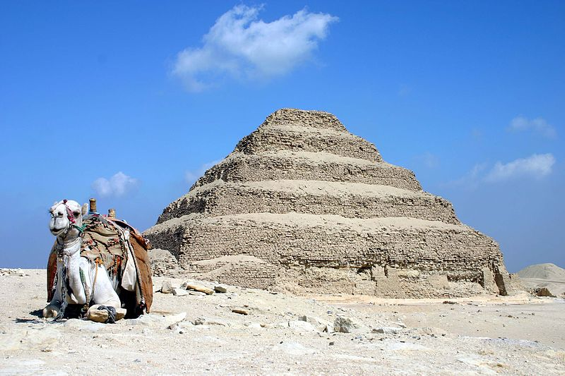
\includegraphics[width=0.4\textwidth]{images/step-pyramid}
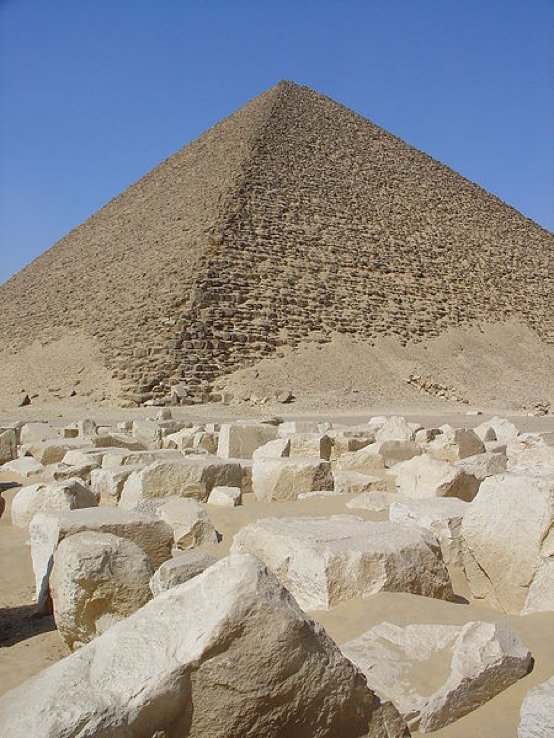
\includegraphics[width=0.4\textwidth]{images/pyramid}
\end{center}

{\scriptsize Source of Left image: Charlesjsharp, Right image: Ivrienen}

\end{frame}



\begin{frame}
\frametitle{Civil Engineering is Hard}

Evidence of errors in civil engineering go back to antiquity

\begin{center}
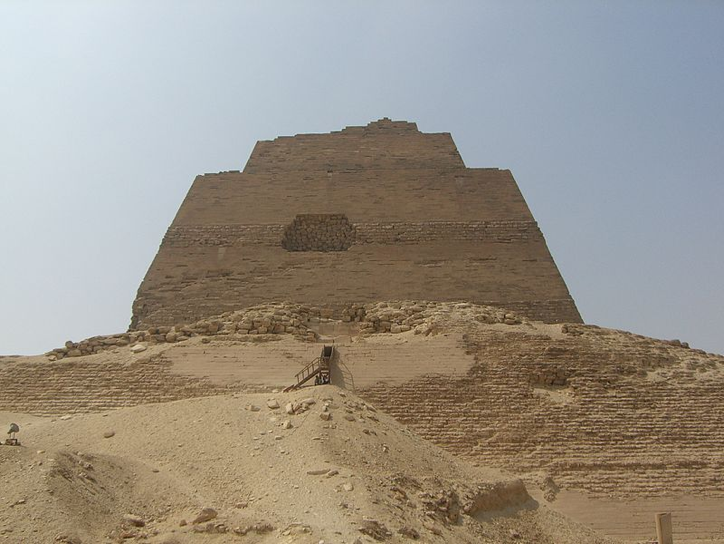
\includegraphics[width=0.4\textwidth]{images/pyramid-fail}
\end{center}

The Meidum pyramid\footnote{\url{http://www.ancientegyptonline.co.uk/pyramid-meidum.html}} (image credit: Neithsabes).


\end{frame}

\begin{frame}
\frametitle{Civil Engineering is Hard}

Evidence of errors in civil engineering go back to antiquity

\begin{center}
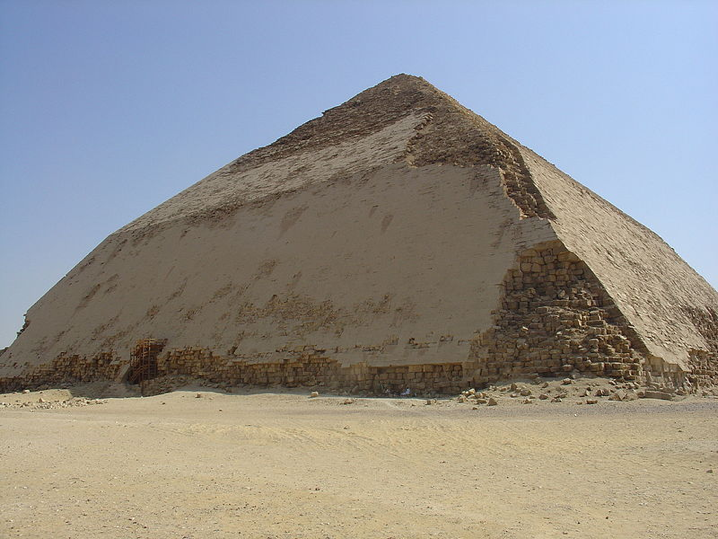
\includegraphics[width=0.4\textwidth]{images/pyramid-bent}
\end{center}

The Bent pyramid (image credit: Ivrienen).


\end{frame}



\begin{frame}
\frametitle{The Code of Hammurabi}

The Code of Hammurabi recognizes a number of professions and places requirements on their work.

\begin{quote}
	228.	If a builder build a house for some one and complete it, he
		shall give him a fee of two shekels in money for each sar of
		surface.
\end{quote}

\begin{quote}
	229.	If a builder build a house for some one, and does not
		construct it properly, and the house which he built fall in
		and kill its owner, then that builder shall be put to death.
\end{quote}

\begin{quote}
	233.	If a builder build a house for some one, even though he
		has not yet completed it; if then the walls seem toppling,
		the builder must make the walls solid from his own means.
\end{quote}

\end{frame}



\begin{frame}
\frametitle{The Code of Hammurabi}

Some additional excerpts from the code:

\begin{quote}
224.	If a veterinary surgeon perform a serious operation on an
		ass or an ox, and cure it, the owner shall pay the surgeon
		one-sixth of a shekel as a fee.
\end{quote}


\begin{quote}
	225.	If he perform a serious operation on an ass or ox, and kill it,
		he shall pay the owner one-fourth of its value.
\end{quote}


\end{frame}

\begin{frame}
\frametitle{The Code of Hammurabi}

Some additional excerpts from the code:

\begin{quote}
215.	If a physician make a large incision with an operating knife
		and cure it, or if he open a tumor (over the eye) with an
		operating knife, and saves the eye, he shall receive ten
		shekels in money.
\end{quote}


\begin{quote}
	218.	If a physician make a large incision with the operating
		knife, and kill him, or open a tumor with the operating knife,
		and cut out the eye, his hands shall be cut off.
\end{quote}


\begin{quote}
	221.	If a physician heal the broken bone or diseased soft part of
		a man, the patient shall pay the physician five shekels in 			money.

\end{quote}


\end{frame}

\begin{frame}
\frametitle{The Code of Hammurabi}

Some additional excerpts from the code:

\begin{quote}
	234.	If a shipbuilder build a boat of sixty gur for a man, he shall
		pay him a fee of two shekels in money.
\end{quote}


\begin{quote}
	235.	If a shipbuilder build a boat for some one, and do not make
		it tight, if during that same year that boat is sent away and
		suffers injury, the shipbuilder shall take the boat apart and
		put it together tight at his own expense. The tight boat he
		shall give to the boat owner.
\end{quote}

\end{frame}



\begin{frame}
\frametitle{Hippocratic Oath}

The Hippocratic Oath comes from Greek and though modified to reflect modern times, is still used in medical schools today.

Famous for the phrase ``first, do no harm'', those words do not actually appear in it.

Excerpt~\cite{hippocratic}:
\begin{quote}
I will use treatment to help the sick according to my ability and judgment, but never with a view to injury and wrong-doing.
\end{quote}



\end{frame}



\begin{frame}
\frametitle{Hippocratic Oath}

The oath also contains references to conflict of interest and confidentiality~\cite{hippocratic}:

\begin{quote}
Into whatsoever houses I enter, I will enter to help the sick, and I will abstain from all intentional wrong-doing and harm, especially from abusing the bodies of man or woman, bond or free. And whatsoever I shall see or hear in the course of my profession, as well as outside my profession in my intercourse with men, if it be what should not be published abroad, I will never divulge, holding such things to be holy secrets.
\end{quote}

\end{frame}



\begin{frame}
\frametitle{Early Professions}


The three ``original'' \textit{learned professions} were divinity, medicine, and law.


There has always been a strong association between higher learning and professions versus trades:
\begin{itemize}
\item It became a full-time occupation
\item The first training school was established
\item The first university school was established
\item The first local association was established
\item The first national association was established
\item The codes of professional ethics were introduced
\item State licensing laws were established
\end{itemize}

\end{frame}



\begin{frame}
\frametitle{Properties of Professions}

A profession will:

\begin{itemize}
\item Use specialized knowledge
\item Require long and intensive preparation
\item Require instruction in skills and methods
\item Be based on scientific, historical or scholarly principles
\item Be maintained by force of organization
\item Hold high standards of achievement and conduct
\item Require continued study
\item Provide service to the public
\end{itemize}


\end{frame}



\begin{frame}
\frametitle{Engineering}

So how did engineering get to be in the list of learned professions?

We have seen that civil engineering goes back to the earliest civilizations.

Ancient civilizations also often had complex military equipment such as artillery, catapults, etc., which were themselves often designed by engineers.

Over time new technologies and new fields of study have caused the profession to expand... software engineering, mechatronics, biomed... 

\end{frame}



\begin{frame}
\frametitle{What is Engineering?}

One definition:

\begin{quote}

The application of scientific, technological, algorithmic, and mathematical principles to make practical use of the properties of matter and sources of energy for the design, manufacture, evaluation, operation and maintenance of engines, machines, structures, devices, materials, systems or processes typically in such a way to be made useful, efficient, and economical for public or commercial purposes.

\end{quote}

\end{frame}



\begin{frame}
\frametitle{What is a Professional Engineer?}

Definition:

\begin{quote}
A \alert{professional engineer} is a person who holds a licence to engage in any act of planning, designing, composing, evaluating, advising, reporting, directing or supervising that requires the application of engineering principles and concerns the safeguarding of life, health, property, economic interests, the public welfare or the environment, or the managing of any such act.
\end{quote}


\end{frame}



\begin{frame}
\frametitle{How Did We Get Here?}

\begin{center}
	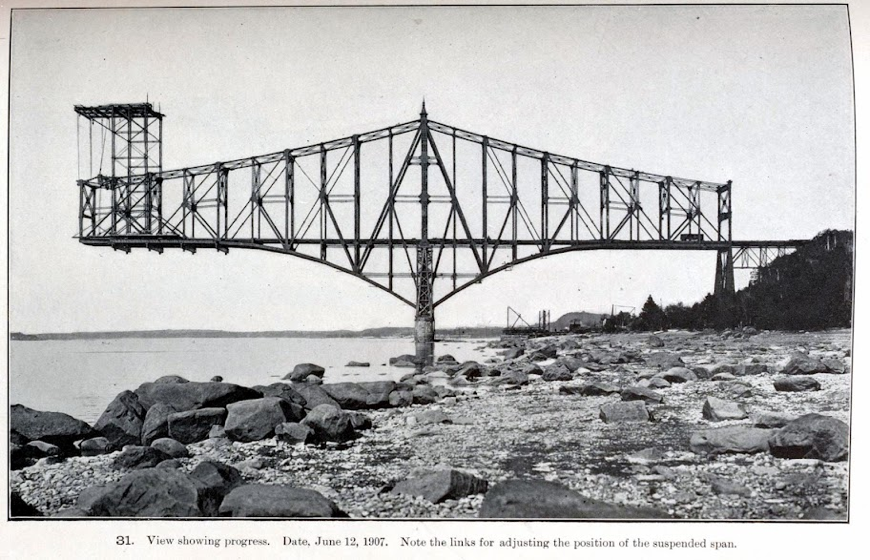
\includegraphics[width=0.8\textwidth]{images/railway-bridge}
\end{center}

The Qu\'ebec Railway Bridge... Before...

\end{frame}

\begin{frame}
\frametitle{How Did We Get Here?}

\begin{center}
	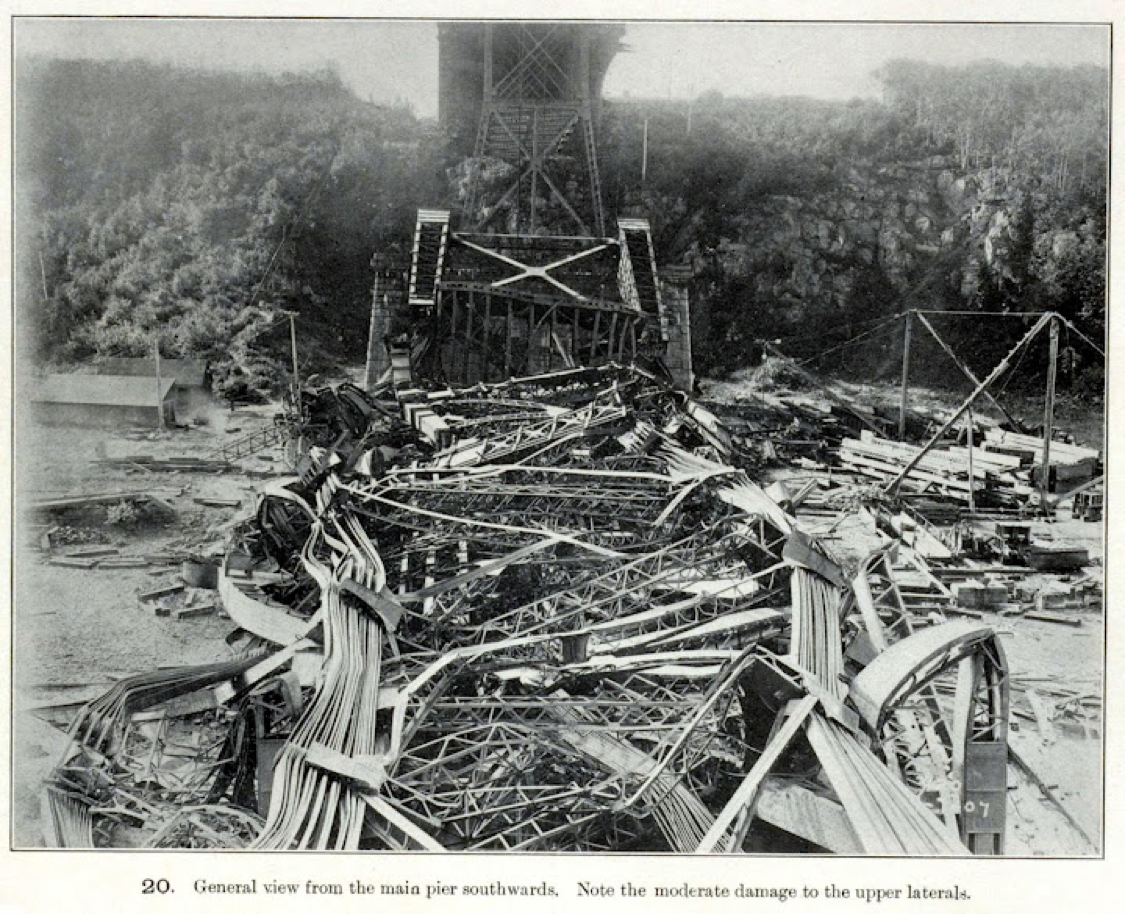
\includegraphics[width=0.75\textwidth]{images/railway-bridge2}
\end{center}

The Qu\'ebec Railway Bridge... After

\end{frame}



\begin{frame}
\frametitle{Railway Bridge is Falling Down...}

This disaster caused engineers in Canada to organize into associations.

The Ontario Government passed the Professional Engineers Act, but membership was voluntary.

Following a series of incidents in the 1930s, membership became mandatory.

In the next lecture we will examine the Professional Engineers Act and the idea of self-regulation in more detail. 

\end{frame}



\begin{frame}
\frametitle{Engineering FAIL}



Tacoma Narrows Bridge: one of the most famous engineering disasters ever.

\begin{center}
	\url{https://www.youtube.com/watch?v=j-zczJXSxnw}
\end{center}

\end{frame}



\begin{frame}
\frametitle{Therac-25}

\begin{center}
    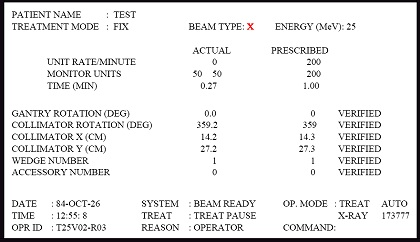
\includegraphics[width=.8\linewidth]{images/Xraybad}
\end{center}

\end{frame}



\begin{frame}
\frametitle{Therac-25}

The issue with electrical and computer engineering is that the product is essentially invisible.

The consumer can only infer what is happening by its response.

This can lead to confusion which you must be ready to address.

Therac-25: Three patients died as a result of the problems with the system!

\end{frame}



\begin{frame}
\frametitle{Therac-25}

\begin{itemize}
	\item \textbf{Race Condition}: A race condition existed between the operator interface task and the equipment control task. This did not occur in testing because AECL did not expect that operators would enter commands in such a quick succession. As operators became more proficient with the system, they entered the commands faster.
	\item \textbf{Overflow}: A flag was incremented and an overflow caused the software to bypass the normal safety checks.
	\item \textbf{Interlocks}: The maximum power setting was enabled without the thick metal plate being in place.
	\item \textbf{Incorrect Feedback}: Although patients had received a fatal amount of radiation, the machine showed that the machine had not delivered the prescribed dose, causing operators to deliver another dose.
\end{itemize}

\end{frame}



\begin{frame}
\frametitle{More Engineering Failure}

There are plenty of other engineering failures for discussion...


\end{frame}

\begin{frame}
\frametitle{References \& Disclaimer}
\bibliographystyle{alphaurl}
\setbeamertemplate{bibliography item}{\insertbiblabel}
{\scriptsize
\bibliography{290}
}
\vfill

{\tiny Disclaimer: the material presented in these lectures slides is intended for use in the course ECE~290 at the University of Waterloo and should not be relied upon as legal advice. Any reliance on these course slides by any party for any other purpose are the responsibility of such parties.  The author(s) accept(s) no responsibility for damages, if any, suffered by any party as a result of decisions made or actions based on these course slides for any other purpose than that for which it was intended.\par}


\end{frame}


\end{document}

